\chapter{Introduction}
\label{:intro}

Range searching is one of the most common types of problems which arise in everyday computer use. 
With a range search, we are given a set of objects and asked to identify those which satisfy some bounded criteria. 
Range searches can take many different forms: searching for email received between two dates, looking for restaurants near your present location, or identifying what a video game player should see on their screen in any one frame; these are all examples of range searches.

In computational geometry, range searching takes on a more abstract quality. 
Typically we are given an environment containing a set of geometric objects such as points, lines, circles, or boxes. 
A query is itself another well-defined geometric object, and our goal is to identify all elements of the environment contained within the query region.  
When addressing a range searching problem, we want to develop a method for preprocessing the input environment so that we can answer any query as efficiently as possible.
Given how common and flexible range searching is to such a wide range of practical computer science, it is not surprising to find that a great deal of research has been expended in this area.  

In this thesis, we address the notion of \emph{Partial Enclosure Range Searching (\PERS{})}, which, to the best of our knowledge, has not been explored previously. 
In this setting, our goal is to identify, for a given query region, all objects which satisfy the \emph{Partial Enclosure Property}, which specifies that an object must intersect a query region by at least some fixed proportion of the object's own size (e.g., length, area, volume) in order to be selected.

This chapter is organized as follows.
Section~\ref{:intro:motivation} begins by describing our motivation for this problem. 
In Section~\ref{:intro:problems} we describe the specific variations of the \PERS{} problem that we will address in this thesis. 
In Section~\ref{:intro:related}, we discuss related problem domains, and contrast them to our own.
Section~\ref{:intro:contributions} outlines the contributions made by this thesis.
We conclude the introduction by outlining the organization of the remainder of the thesis in Section~\ref{:intro:organization}.


%------------------------------------------------------------------------------
%------------------------------------------------------------------------------
\section{Motivation}
\label{:intro:motivation}

This problem was inspired by the author's use of Microsoft OneNote. 
Using a digital pen, OneNote can be used much like a paper notebook, allowing the user to add handwriting, diagrams, equations, and any other such thing to a page.
Unlike a paper notebook, OneNote also allows the user to select previously drawn objects in order to translate, scale, copy and otherwise manipulate them.
Figure~\ref{fig:intro:onenote} shows some handwritten notes, and a diagram which has been partially selected.

\begin{figure}
\begin{center}
  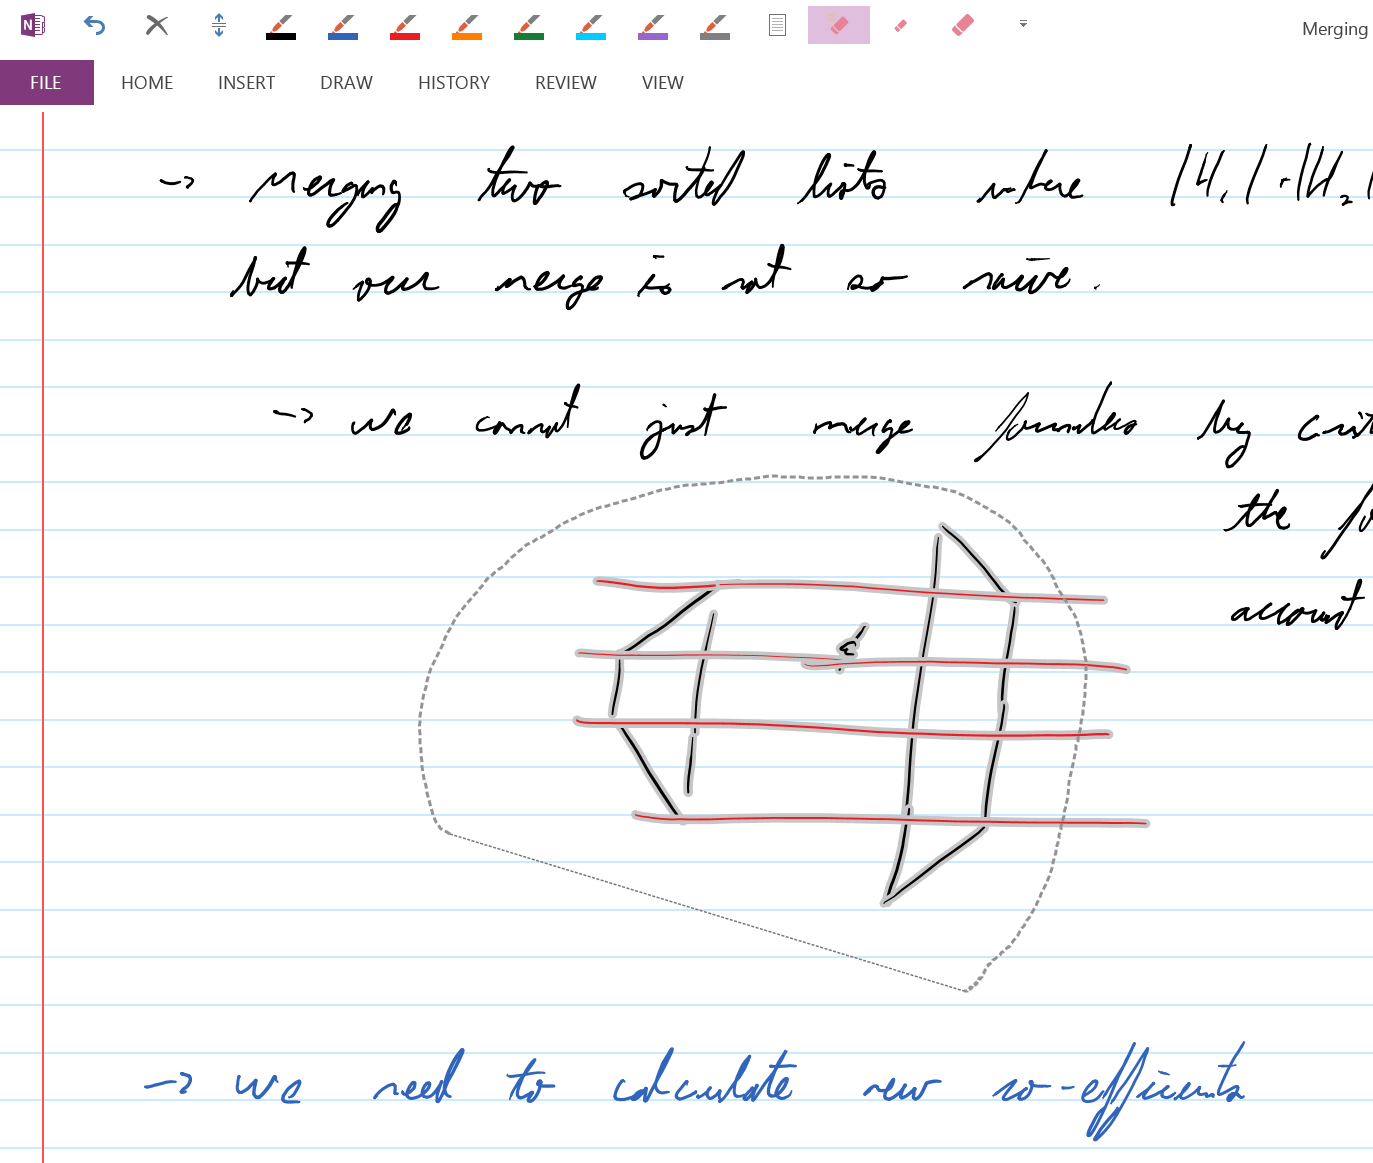
\includegraphics[width=0.50\textwidth]{figures/fig_onenote}
  \caption[An example of practical partial enclosure range searching]{An example of practical partial enclosure range searching in Microsoft OneNote. The line segments in the middle are selected even though they are not entirely enclosed.}
  \label{fig:intro:onenote}
\end{center}
\end{figure}

Looking carefully at the figure, we can see that even though the horizontal line segments of the diagram have not been entirely enclosed by the selection tool, they nevertheless appear as part of the set of selected items.
This behaviour of selecting partially enclosed objects is described in a patent filed by Microsoft Corporation\cite{lassoselect}. 
From the patent:

\begin{quote}
[T]here is a need for a selection tool that will allow a user to conveniently select one or more graphical objects in their entirety, without requiring an inconvenient amount of precision from the user.
\end{quote}

\noindent With the rising popularity of touch and pen-enabled devices, this need is likely to increase.  
As we can see from the figure, OneNote already includes an implementation of a partial selection tool like the one described by the patent. 
Although the details of the implementation are proprietary, it becomes apparent while using the software that it suffers from poor performance as more items are selected.
It is from this observation that the work in this thesis was inspired.  
Although the problems that we will examine take place in simpler settings than the patent describes, we will nevertheless develop an understanding of the major challenges of this problem domain, as well as some techniques for addressing them.


%------------------------------------------------------------------------------
%------------------------------------------------------------------------------
\section{Problem Statements}
\label{:intro:problems}

This thesis proposes algorithms for several different partial enclosure range search settings.  Each problem addresses a different type of geometric object to be queried, or a different type of query region.

\paragraph{Line Segments and Query Rectangles.} Line segments and rectangles are one of the simplest settings in which we can perform partial enclosure range searches. 
Given an axis-parallel query rectangle, we address methods which consider only axis-parallel segments, or which consider arbitrarily-oriented ones.

\paragraph{Line Segments and Query Slabs.} Relaxing the axis-parallel query regions of the preceding problem, we consider an arbitrarily-oriented slab.
As the query slab can have any orientation, intersections with a horizontal segment will involve both the height of the segment and the slope of the slab.  
We also consider a query defined as the intersection of two slabs.

\paragraph{Convex Polygons and Query Rectangles.} Moving away from line segments, we consider problems of partial enclosure with respect to area.  
For any such problem, deciding on the partial enclosure property is straight-forward once we know the area of the input object and the area enclosed by a query region.  
We consider how to determine the proportion of a convex polygon enclosed by a query rectangle.
 
\paragraph{Monotone Polygons and Query Rectangles.} This more complex shape does not generally decompose into big convex regions, so a different method of preprocessing will be needed.
We consider methods for calculating the area of the polygon to one side of a query line. 
With such a method in hand, determining the area of a rectangle is a matter of executing several queries and combining their results.

%------------------------------------------------------------------------------
%------------------------------------------------------------------------------
\section{Related Work}
\label{:intro:related}

In this section, we review some existing variations of the range searching problem.
As a whole, due to its applicability to such a wide assortment of problems, range searching has received a great deal of research attention.
Aside from the solutions to specific problems that this research has found, it has also resulted in a vast toolbox of observations and techniques, many of which apply to our own problem.

Range searching structures are typically constructed by subdividing the input objects, or the space in which the input objects exist, into several regions which express useful properties.
Ideally, we are able to choose these regions so that a query area will entirely contain, or not contain, most of these regions, while intersecting only a small number of them.
On those intersected regions, we continue the query on the recursively finer subdivisions stored there.\cite{Matousek93}

This recursive decomposition into regions which is employed by many techniques has an extremely beneficial side-effect. 
At each region in this hierarchy, we can associate any other structure of our choosing.
These so-called multi-level structures can be used to answer complex queries by using the outer structure to find objects satisfying one query parameter, and then continuing with the associated structures to find objects which satisfy additional properties.
We discuss examples of this type of multi-level query in detail in Chapter~\ref{:prelim}.

The remainder of this section gives a brief introduction to some specific range searching problems, and history of some methods for answering each. 
We refer the reader to an excellent survey on range searching by Agarwal and Erickson\cite{Agarwal99} for a more detailed introduction.


\subsection*{Orthogonal Range Searching} 

In its general form, an orthogonal range searching problem starts with a set $S$ of points in $\mathbb{R}^d$, where $d$ is a small, fixed constant.
A query is a $d$-dimensional, axis-parallel box, and our goal is to identify the subset of our input points which are contained within this box.

\emph{Quadtrees}, first described by Finkel and Bentley\cite{Finkel74} (see also \cite[Chapter~14]{Deberg}), are one of the very first structures for performing range searches.
When we are considering points in the plane, a quadtree works by dividing the space containing the points into squares, and then recursively splitting any region which contains more than one point into four smaller, but equally-sized squares.

Because this recursion is based on splitting space rather than the points within the space, the recursion depth, and thus the depth of the quadtree, is not related to the number of points. 
Instead, the size of the initial square from which we start splitting and the distance between the closest pair of points are the important factors.
For an initial square with a side length of $s$ and a closest pair with distance $c$, the recursion depth is $\BigOh{\log{\frac{s}{c}}}$.
The construction and query times are related to this recursion depth, making the structure somewhat slow, but it \emph{does} work!

Quadtrees can be easily extended to work in higher dimensions. 
In $\mathbb{R}^3$ quadtrees are called \emph{Octrees}, and the general method can be extended to even higher dimensions. 
For points and an initial box in $\mathbb{R}^d$, decomposition proceeds along the same basic rules, but using progressively smaller $d$-boxes instead of just squares.


KD-Trees\cite{Bentley75} were the first major improvement over quadtrees.
Unlike a quadtree which partitions space, a KD-Tree directly partitions the pointset in a recursive manner.
For points in the plane, each level of the tree corresponds to a particular axis.
Suppose that we start with the $x$-axis at the root level.
We consider the median point $m$ with respect to the $x$-coordinates of all the points, and then all remaining points are partitioned as left or right of this vertical \emph{splitting line} through $m$.

On the next level of the recursion we alternate to the $y$-axis, select the median point with respect to $y$-coordinates, and partition around the horizontal splitting line through that point.
The process continues, alternating the axis on each level, until we create leaves containing single points.
This process creates a balanced tree, where each path through the tree alternates between axes.
Each node in the tree represents a region of the plane bounded by its own splitting line and the splitting lines of its ancestors.

Querying a KD-Tree by a rectangular region involves traversing the tree while only visiting those nodes whose region is intersected by the query region.
While the preprocessing requirements of a KD-Tree are quite good, at $\BigOh{n}$ space and $\BigOh{n\log{n}}$ preprocessing time, the query time is $\BigOh{\sqrt{n}}$.

A final note about KD-trees, this recursive construction can be generalized to higher dimensions in a straight-forward manner, by simply cycling through each of the $d$ axes in order.
The preprocessing requirements are unchanged asymptotically, since we still create just a single binary tree with $n$ leaves.
The query algorithm is also similar to the $\mathbb{R}^2$ case, but with a query time of $\BigOh{n^{1-1/d}}$.

The next improvement in orthogonal range searching came in the form of a polylogarithmic method known as \emph{Range Trees}. 
Range trees were discovered by Bentley\cite{Bentley79}, who was involved in the last two structures, but were also simultaneously developed by other independent researchers.
This method is constructed on binary search trees and can query any open or closed query box in $\BigOh{\log^{d-1}{n}}$ time with only $\BigOh{\log^{d-1}{n}}$ time and space pre-processing.
We discuss this structure in more detail in Section~\ref{:prelim:range-trees}.

%Best known by Chazelle [Dutch 90,91] in 2D and higher dimensions with time/space of XXX

Finally, a noteworthy special case occurs when our points are in the plane and our query is a three-sided rectangle, i.e., when it is open to one side.
In this case, we can use a method developed by McCreight\cite{McCreight85} which gives $\BigOh{\log{n} + k}$ query time, where $k$ is the number of points found, while using only $\BigOh{n}$ space and $\BigOh{n\log{n}}$ preprocessing time.

The real power of orthogonal range searching is in how other problems can be reduced to instances of it by encoding query keys as coordinates of a high-dimensional point.  
For example, in the geometric sense, we can search for rectangles inside of rectangles by mapping the coordinates of an input rectangle in $\mathcal{R}^{d}$ to a point in $\mathcal{R}^{2d}$, and performing an orthogonal range search in that space.
Rectangle-in-rectangle queries are important as rectangles make easy approximations of more complicated geometric objects that we may want to look for.

Outside of purely geometric applications, many more general types of range searching problems can be similarly reduced to instances of orthogonal range searching.
For example, given some integer representation of a date, we can search for emails received within a date range by encoding the date stamp of each email into a point, and then searching for points between the two integer representations of our query range.
Extending this idea to more complex queries is just a matter of mapping each key we wish to search on to further components of a higher-dimensional point.  
In this way, multi-dimensional orthogonal range searching can be used to perform multi-key searching.\cite{Willard96} 


\subsection*{Half-plane Range Searching}

In general, when performing half-plane queries, we need to make a choice between using a structure which has low space or one with a fast (polylogarithmic) query time.
We introduce a structure suitable for each side of this trade-off.

If we want to save space, we can use a \emph{Ham Sandwich Cut Tree}\cite{Edelsbrunner86, Edelsbrunner87}.
To construct this tree, we divide all of our points into four quadrants of equal size, which we accomplish with an algorithm by Megiddo\cite{Megiddo85} in $\BigOh{n}$ time.
We continue construction by repeating this process on each quadrant recursively, and building a tree out of the results of each step.
The final tree has size $\BigOh{n}$ and is constructed in $\BigOh{n\log{n}}$ time.

We can query this tree with the line representing the boundary of a query half-plane.
The quadrants at any step are the result of two intersecting lines. 
Their intersection point must be on or to one side of any query line, and thus, the query line will intersect at most three quadrants.
The non-intersected quadrants must then be either entirely inside the query half-plane, or entirely outside of it.
The query then recurses on the intersected quadrants.
Total query time is $\BigOh{n^{\log_2(1 + \sqrt{5}) - 1}} \approx \BigOh{n^{0.695}}$.


If we want to save query time, then we can use a \emph{Level Arrangement}\cite{GoswamiDN04}.  
This structure has a query time of only $\BigOh{\log{n}}$ but requires $\BigOh{n^2}$ storage.
The level arrangement structure is constructed in a dual space.
Given a set $S$ of $n$ points $p_1, p_2, \ldots, p_n$ where each $p_i = (a_i, b_i)$, we map each point to a corresponding dual line $l_i: y = a_i \cdot x - b_i$.

Considering all of the intersection points formed by the set of dual lines crossing each other, and the edges between them, we can easily see the $\BigOh{n^2}$ size.
Preprocessing continues by enclosing the environment in a bounding box which contains all of the intersections.
By following the monotone chains of intersections from left to right, we can determine the ``level'' of each edge, that is, the number of edges below (or above) each edge.
Total preprocessing time is $\BigOh{n^2}$.

In this dual space, the line which defines the boundary to our query half-plane becomes mapped to a point.
The query proceeds by selecting the median level of the arrangement, and then performing a binary search over its edges to find the one above or below the query point.
This process is repeated in a binary search sort of fashion on the subset of levels containing the query point until we have found the levels directly above and below the query point. 
Depending on the half-plane, the levels lying to one side of the query point or the other correspond to the input points satisfying the query half-plane.
As we have described it here, this query requires $\BigOh{\log^2{n}}$ time, but this can be reduced to $\BigOh{\log{n}}$.\cite{NandyDG03}

A different approach to solving half-plane range searches altogether is to consider a half-plane as a degenerate simplex, and then use any simplex range searching structure to answer a query.  
Such structures are discussed below and in Section~\ref{:prelim:chan}.

One final method for half-plane searches we would like to mention is by Chazelle \emph{et al.}\cite{ChazelleGL85,Chazelle85} as it does not obey the general trade-off between space and query time that we mentioned above.
This method uses \emph{convex layers} and gives $\BigOh{n}$ storage and $\BigOh{\log{n} + k}$ query time, where $k$ is the number of points found. 

Convex layers of a pointset are easiest to explain by their construction, which is performed iteratively by calculating the convex hull, deleting it, and then taking the convex hull of what remains, until all points are deleted.
Convex layers can be constructed in $\BigOh{n\log{n}}$ time, and require $\BigOh{n}$ space.
In order to use convex layers for half-plane queries, we will translate the pointset such that the origin point of the plane occurs inside the innermost convex layer.

A query line which passes through the pointset will intersect some or all of the layers, from $l_1$ at the outside to $l_m$, the innermost layer which is intersected.
The query is performed in two main steps: identify $l_m$, and then report all of the points.

Locating $l_m$ is done in a dual space transformation.
Our pointset becomes an arrangement of lines, and our query line becomes a point.
A consequence of the origin point being inside the innermost convex layer in the primal space is that the dual space will be comprised of corresponding levels, although in reverse order.
We can then perform any planar point location method we like on the query point to determine the level containing it; Chazelle \emph{et al.} give several $\BigOh{\log{n}}$ choices.

With the convex layer $l_m$ known, we can compute the intersections of the query line with $l_m$ in $\BigOh{\log{n}}$ time, and in so doing, identify at least one point which is inside our query half-plane.
During preprocessing, we augment every vertex with pointers to the edges which appear above and below them in neighbouring convex layers, accomplished by walking around two neighbouring layers at a time simultaneously.
Depending on which side of the query line our half-plane extends, we can walk these pointers from $l_m$ across the remaining levels, whether that first takes us deeper into the layers, or directly out.
At each level, we then traverse left and right around the level for as long as we remain in the query half-plane reporting our matching points.


\subsection*{Simplex Range Searching}

In simplex range searching in the plane, there is no known data structure which can answer a query in polylogarithmic time using linear (or nearly linear) storage.\cite{Agarwal99}  

Considering structures with linear or near linear storage, the first sublinear query time algorithm in this area was by Willard in 1982\cite{Willard82}.
His paper introduced a method using \emph{partition trees}.
The general idea is to partition space into several regions each containing a roughly equal number of input points.
Each region is then recursively built in the same way.
The goal is to choose our regions in such a way that the largest number of regions which may be intersected by any line is minimized.  
This property is known as the \emph{crossing number}.
Willard's approach requires a query time of $\BigOh{n^{0.774}}$.
Moreover, the partition tree approach in general expresses a ``nice'' recursive structure which lends itself to multi-level query structures.

Following this first approach, a series of improvements were made to the partition tree method, mostly concentrating on developing a lower crossing number.
For many years, the best known approach was by Matousek\cite{Matousek92} which requires $\BigOh{n\log{n}}$ preprocessing time and $\BigOh{\sqrt{n}\log^{\BigOh{1}}{n}}$ query time.
Recently, this has been improved to a query time of just $\BigOh{\sqrt{n}}$ by Chan\cite{chan2012} with the same preprocessing time.
We use this latter method throughout Chapters \ref{:rectangles} and \ref{:slabs}, and discuss it in more detail in Section~\ref{:prelim:chan}.


\subsection*{Intersection Searching} 

Intersection searching is similar to range searching, except that we consider different types of geometric input objects aside from points.
Given a query region, we are looking for any objects which have even a single point of intersection in common with the query itself; that is, the object need not be entirely enclosed with the query region.
In this way, we can think of range searching as a specialization of intersection searching.
We introduce just a few of the many variations of intersection searching problems.

In \emph{Segment Intersection Searching}, the query is a line segment. 
The case where both the input objects and the query are orthogonal line segments has many applications in VLSI design.
Orthogonal or otherwise, segment intersection searching can be efficiently solved using plane-sweep algorithms.

\emph{Rectangle Intersection Searching}, also known as \emph{Windowing Queries} identify polygons which intersect a rectangular query region. 
Many computer graphics problems are related to this problem as, for example, we might want to determine what items need to be rendered on screen from a 3D environment.

Finally, \emph{Point Intersection Searching} is sort of the opposite of a normal range searching query. In this problem, we are interested in reporting all objects which contain a query point.

Some of these methods, notably windowing queries, initially seemed as though they would be helpful in solving \PERS{} problems.
For example, looking at our line segment problems, we could start by considering only those segments that at all intersect a query region, and then perform additional steps to identify only those which are sufficiently enclosed.
However, in the worst case, the number of segments intersecting the query region could be much, much higher than the number satisfying the partial enclosure property, such that the added steps of the intersection query do not help at all.


\subsection*{Completing a Search}

Throughout this section, we've used the term ``identify'' rather loosely.
For the hierarchical structures above, ``identifying'' points satisfying a query really comes down to isolating those partitions, or disjoint subsets, which contain them.
What we do with the partitions at that point is somewhat flexible.
For example, we can simply count the points we have identified with only a constant factor of extra time and space by having the partitions store their own sizes.
We could instead report the points by traversing the contents of the partition, although this will cost us an extra linear factor with respect to to the number of reported items.
We use the term ``identify'' in this way throughout the thesis.

We conclude this section by comparing and contrasting our own problem with the ones we have just introduced.

Our problem is notably different from standard range searching problems because we are not just looking for items which are entirely contained inside of a query region.
This immediately rules out a simple application of orthogonal range searching like we saw with the rectangles-in-rectangles problems.

Our problem also differs from intersection searching, since we have the extra constraint of requiring a specific proportion of the input objects to be contained in the query region, rather than just any point.


%------------------------------------------------------------------------------
%------------------------------------------------------------------------------
\section{Summary of Contributions}
\label{:intro:contributions}

In this thesis, we develop contributions to several variations of the \PERS{} problem, along with some noteworthy ancillary methods. 
Table~\ref{tab:contributions} gives a broad overview of these techniques. 
The table uses `AP' for ``Axis-Parallel'', `AO' for ``Arbitrary Orientation'', `P' for ``Polygon'', and omits ``Big Oh'' for clarity.

\begin{table}[t]
\caption{Summary of Contributions}
\label{tab:contributions}
\centering
\begin{tabular}{l l l l l l}
\hline \hline
Object & Query & Theorem & Space & Time & Query \\
\hline
AP Segment & AP Rectangle & Th~\ref{th:ap} & ${n\log^3{n}}$ & ${n\log^3{n}}$ & ${\log^3{n}}$ \\
AO Segment & AP Rectangle & Th~\ref{th:ao} & ${n\log^7{n}}$ & ${n\log^7{n}}$ & ${\sqrt{n}\log^7{n}}$ \\
AP Segment & AO Slab & Th~\ref{th:slabs:one} & ${n\log^2{n}}$ & ${n\log^3{n}}$ & ${\sqrt{n}\log^3{n}}$ \\
AP Segment & 2 AO Slabs & Th~\ref{th:slabs:two} & ${n\log^3{n}}$ & ${n\log^3{n}}$ & ${\sqrt{n}\log^3{n}}$ \\
Convex P & Rectangle & Th~\ref{th:convexp:area} & ${n}$ & ${n}$ & ${\log{n}}$ \\
Convex P & Convex $k$-gon & Cor~\ref{cor:convexp:karea} & ${n}$ & ${n}$ & ${k \log{n}}$ \\
Monotone P & AP Rectangle & Th~\ref{th:monotonep:rect:area} & ${n\log{n}}$ & ${n\log{n}}$ & ${\log{n}}$ \\
Monotone P & AP Rectangle & Th~\ref{th:mono2} & ${n}$ & ${n\log{n}}$ & ${\sqrt{n}}$ \\
Simple P & Horiz Slab & Cor~\ref{cor:monotonep:simplep-area} & ${n}$ & ${n}$ & ${\log{n}}$ \\
\hline
\end{tabular}
\end{table}

In the line segment cases, we develop methods for restating the partial enclosure property as something which can be evaluated as a one or two variable inequality. 
These expressions can then be queried by known structures for orthogonal or half-plane range searching. 
We discuss the transformations to appropriate dual-spaces and the design of data structures which can answer the necessary multi-part queries.

In the polygon cases, we primarily develop methods for calculating area within a simple region, e.g., below a query line.
These methods are then repeated and combined to find the area enclosed by the actual query region.
Once the enclosed area is known, determining the partial enclosure property is straight-forward.

%------------------------------------------------------------------------------
%------------------------------------------------------------------------------
\section{Organization of the Thesis}
\label{:intro:organization}

The remainder of this thesis is organized in the following way. 
Chapter~\ref{:prelim} reviews existing data structures and range searching techniques which we utilize in our own contributions.
The next four chapters cover partial enclosure range searching queries on successively more sophisticated geometric objects, with Chapter~\ref{:rectangles} focusing on axis-parallel rectangles, Chapter~\ref{:slabs} on arbitrarily-oriented slabs, Chapter~\ref{:convexp} on convex polygons, and Chapter~\ref{:monotonep} on monotone polygons.
The thesis concludes with Chapter~\ref{:conclusion} which summarizes the contributions and future work presented in earlier chapters.
